\begin{wrapfigure}[18]{r}[0pt]{30mm}
	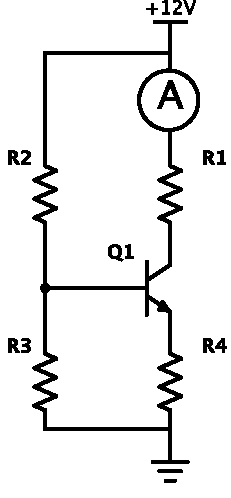
\includegraphics[width=30mm]{cc1.pdf}
	\caption{Sorgente di corrente costante.}
	\label{fig:cc1}
\end{wrapfigure}

\section{Sorgente di corrente costante}
Prima di montare il circuito riportato in Fig. \ref{fig:cc1}, abbiamo dimensionato le resistenze $R_1$ e $R_2$ del partitore in modo da avere una sorgente di corrente costante $I_L=\SI{1}{\milli\ampere}$.
Avendo scelto come $R_E=(997.3 \pm 0.2)\,\si{\ohm}$ e utilizzando la relazione $I_L+I_B=I_E \Rightarrow I_L \approx I_E$ \footnote{Nei transistor la corrente di base è circa 100 volte inferiore rispetto a quella di collettore ed emettitore.} possiamo facilmente calcolare la tensione di base necessaria per fornire una $I_L=1\si{\milli\ampere}$: $V_B=I_L \cdot R_E + 0.6V$.
Il secondo termine deriva dal fatto che tra base ed emettitore, essendo una giunzione p-n, vi è una caduta di tensione pari a $0.6V$.

Risulta immediato impostare dunque l'equazione che permette di calcolare i valori delle resistenze nel partitore:

\begin{equation}
\frac{R_2}{R_1+R_2} V_{CC}=I_L \cdot R_E + 0.6V
\label{partitore}
\end{equation}

Evidentemente i valori delle resistenze non sono univocamente determinati da Eq. (\ref{partitore}).
Sarà dunque nostro compito scegliere una delle due in modo che non venga dissipata troppa potenza sul partitore e contemporaneamente scorra abbastanza corrente attraverso la base del transistor.
È stata scelta $R_1=99.06 \pm 0.01 \,\si{\kilo\ohm}$, valore che ci sembrava adeguato per soddisfare le due caratteristiche sopra citate.

\begin{figure}[H]
\centering
	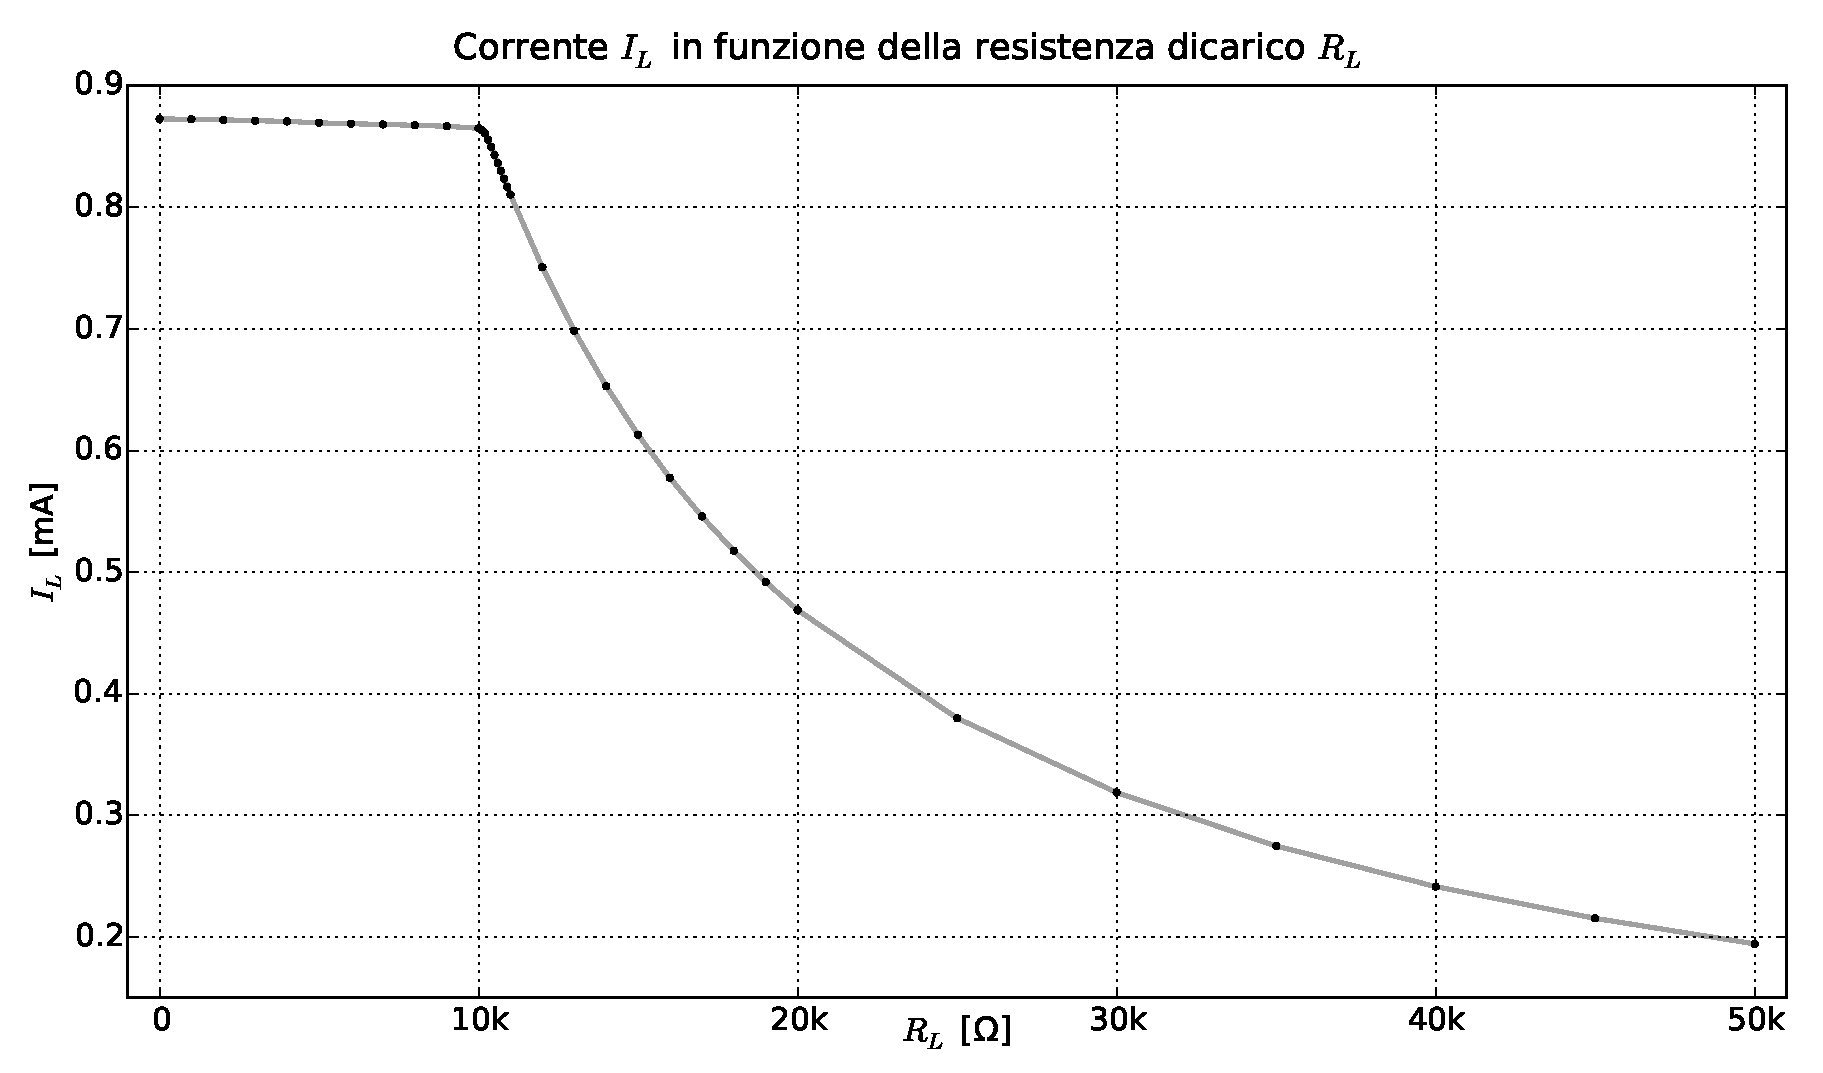
\includegraphics[scale=0.45]{sorgente.pdf}
	\caption{grafico della corrente fornita dalla sorgente di corrente in funzione del carico $R_L$. La linea in verde rappresenta il comportamento ohmico del circuito per $R_L$ elevate.}
	\label{fig:sorg}
\end{figure}

Da Eq. (\ref{partitore}) risulta $R_2 = \SI{18.6}{\kilo\ohm} $.
Il valore effettivamente utilizzato nel circuito è stato $R_2 = (18.01 \pm 0.02 )\,\si{\kilo\ohm} $.
Tale lieve discrepanza non influenzerà certamente la bontà dell'esperimento.
Infatti anche il transistor, in base alla temperatura dell'ambiente, avrà delle variazioni considerevoli delle caratteristiche intrinseche.
Ci aspettiamo dunque che il valore di corrente che successivamente andremo a misurare non avrà un valore esatto di $1\si{\milli\ampere}$. 
Il grafico di $I_L$ in funzione del carico è riportato in Fig. \ref{fig:sorg}.

Ricordiamo anzitutto che avendo avuto una $I_L<\SI{1}{\milli\ampere}$ per qualsiasi carico, abbiamo utilizzato il multimetro in modalità amperometro con un fondo-scala di $\SI{1}{\milli\ampere}$ senza mai cambiarlo (così facendo abbiamo evitato di dover correggere i dati per le diverse resistenze interne dello strumento stesso).

Come si vede graficamente, per valore di $R_L<\SI{10}{\kilo\ohm}$, il valore di corrente di collettore è pressoché costante.
Per valori di $R_L>\SI{10}{\kilo\ohm}$ la corrente decresce.
Ciò è dovuto al fatto che, se la differenza di tensione collettore-emettitore è inferiore a $0.2V$, il transistor entra in saturazione e a quel punto la corrente di  collettore non è più determinata dalla corrente di base ma dal carico $R_L$.
Risulta immediato verificare che  per un valore di carico superiore a $\SI{10}{\kilo\ohm}$ i dati obbediscono alla legge di Ohm.

%**dati del fit e spiegare se è possibile stimare Vce dai dati**   

\begin{wrapfigure}[18]{r}[0pt]{38mm}
	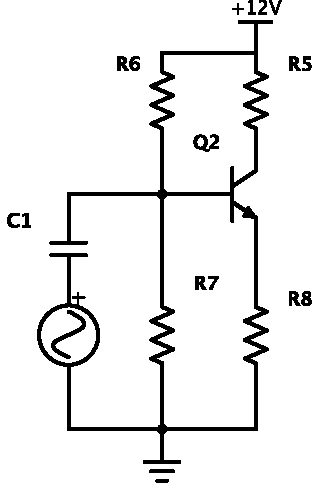
\includegraphics[width=38mm]{cc2.pdf}
	\caption{Amplificatore ad emettitore comune.}
	\label{fig:cc2}
\end{wrapfigure}

\section{Amplificatore ad emettitore comune}

Riportiamo in Fig. \ref{fig:cc2} lo schema del circuito utilizzato per questa seconda parte dell'esperienza.
Anche in questo caso abbiamo dovuto dimensionare le resistenze del partitore e inoltre anche la capacità $C_1$.
Avendo scelto come $R_E=(498.4\pm0.1)\,\si{\ohm}$ e volendo una corrente di quiescenza di $\approx \SI{1}{\milli\ampere}$ abbiamo stimato $V_B=1.1V$.
Possiamo ora, attraverso Eq. (\ref{partitore}), calcolare i valori di $R_1$ e $R_2$.
Avendo anche in questo caso scelto $R_1=(100.03\pm0.2)\,\si{\kilo\ohm}$ abbiamo utilizzato una $R_2=(12.16\pm0.01)\,\si{\kilo\ohm}$.
Come segnale in ingresso è stata usata una forma d'onda sinusoidale a frequenza di $\SI{1}{\kilo\hertz}$.
Per la struttura del circuito risulta semplice impostare il calcolo di $C_1$.
Infatti il condensatore è caricato dal parallelo delle resistenze del partitore.
Inoltre, esso fa parte di una sorta di filtro passa alto.
Basterà dunque utilizzare dei valori di capacità adeguati in modo da avere una frequenza di taglio minore di $\SI{1}{\kilo\hertz}$.
Riportiamo ora l'equazione utilizzata per il calcolo di $C_1$

\begin{equation}
C_1>>\frac{1}{2 \pi \cdot R_1 // R_2}
\end{equation}

Inserendo i nostri valori, otteniamo $C_1>>\SI{15}{\nano\farad}$.
È stato dunque scelto di usare un uno dei primi condensatori trovati sul tavolo con capacità $C_1=(0.982\pm0.005)\,\si{\micro\farad}$.
Per la nostra esperienza era richiesto un guadagno in tensione pari a $G=-10$.
Ricordando che $G\doteqdot \frac{e^{i\pi}R_C}{R_E}$ è stato immediato pickare una $R_C=(4.969\pm0.001)\,\si{\kilo\ohm}$. 

Stimati tutti i valori delle componenti circuitali, abbiamo montato il circuito vero e riportando a schermo dell'oscilloscopio sia segnale in ingresso che in uscita.
Nel seguente grafico sono riportati i dati dell'oscilloscopio.

\begin{figure}[H]
\centering
	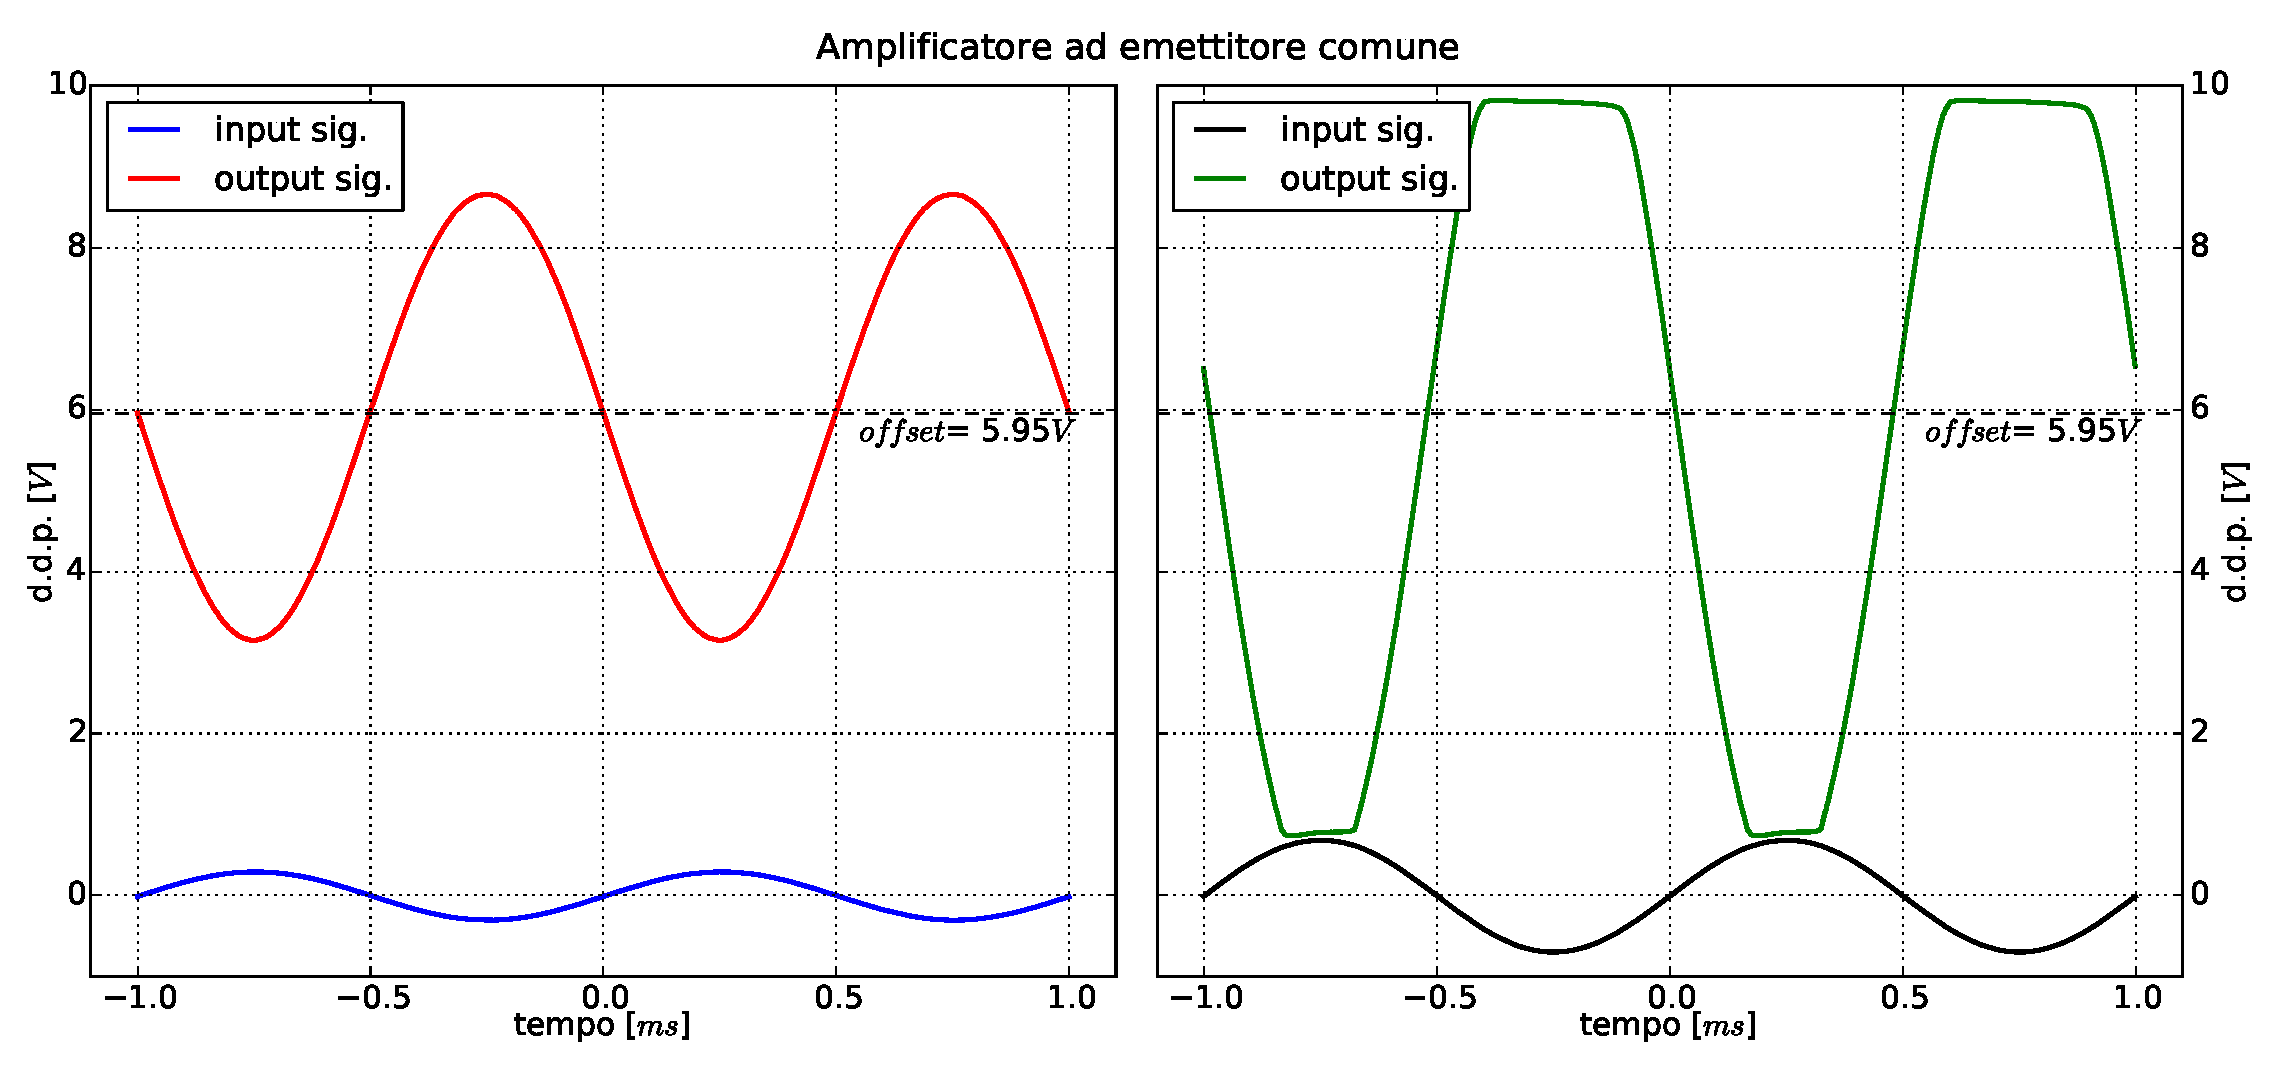
\includegraphics[scale=0.45]{amp.pdf}
	\caption{Amplificatore ad emettitore comune. Nel grafico a sinistra è riportato il comportamento dell'amplificatore nella zona ottimale, mentre nella zona a destra è riportato l'andamento del segnale in uscite nelle condizioni di ``\emph{clipping}''}
	\label{fig:amp}
\end{figure}

Come vediamo immediatamente, il segnale in uscita è sfasato di $\pi$.
Proprio per questo motivo nella formula del guadagno compare quel $e^{i\pi}$.
Dai dati sperimentali è stato possibile stimare il valore di guadagno effettivo, utilizzando la tensione picco-picco:

$$G_{exp}=e^{i 0.9972 \pi} suca$$

\begin{wrapfigure}[18]{r}[0pt]{36mm}
	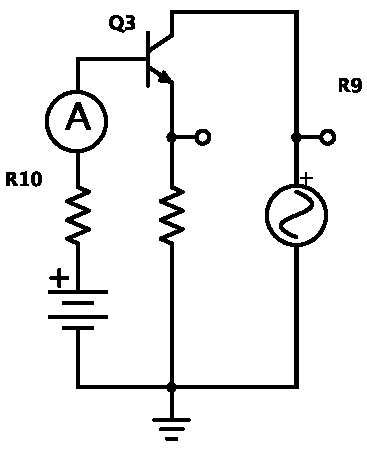
\includegraphics[width=36mm]{cc3.pdf}
	\caption{Sorgente di corrente costante.}
	\label{fig:cc3}
\end{wrapfigure}

\section{Caratteristica di uscita}

In questa ultima parte dell'esperienza abbiamo cercato di analizzare la caratteristica di uscita del transistor.
Per fare ciò abbiamo montato il circuito in Fig. ().
Alimentandolo con un'onda sinusoidale di frequenza $\SI{1}{\kilo\hertz}$, con tensione picco-picco di $10V$ e offset di $+5V \, DC$ e impostando l'oscilloscopio in configurazione XY, possiamo ottenere la caratteristica di uscita per diverse correnti di base (impostate cambiando la $V_B$).

\begin{figure}[H]
\centering
	\caption{Caratteristica di uscita del transistor}
	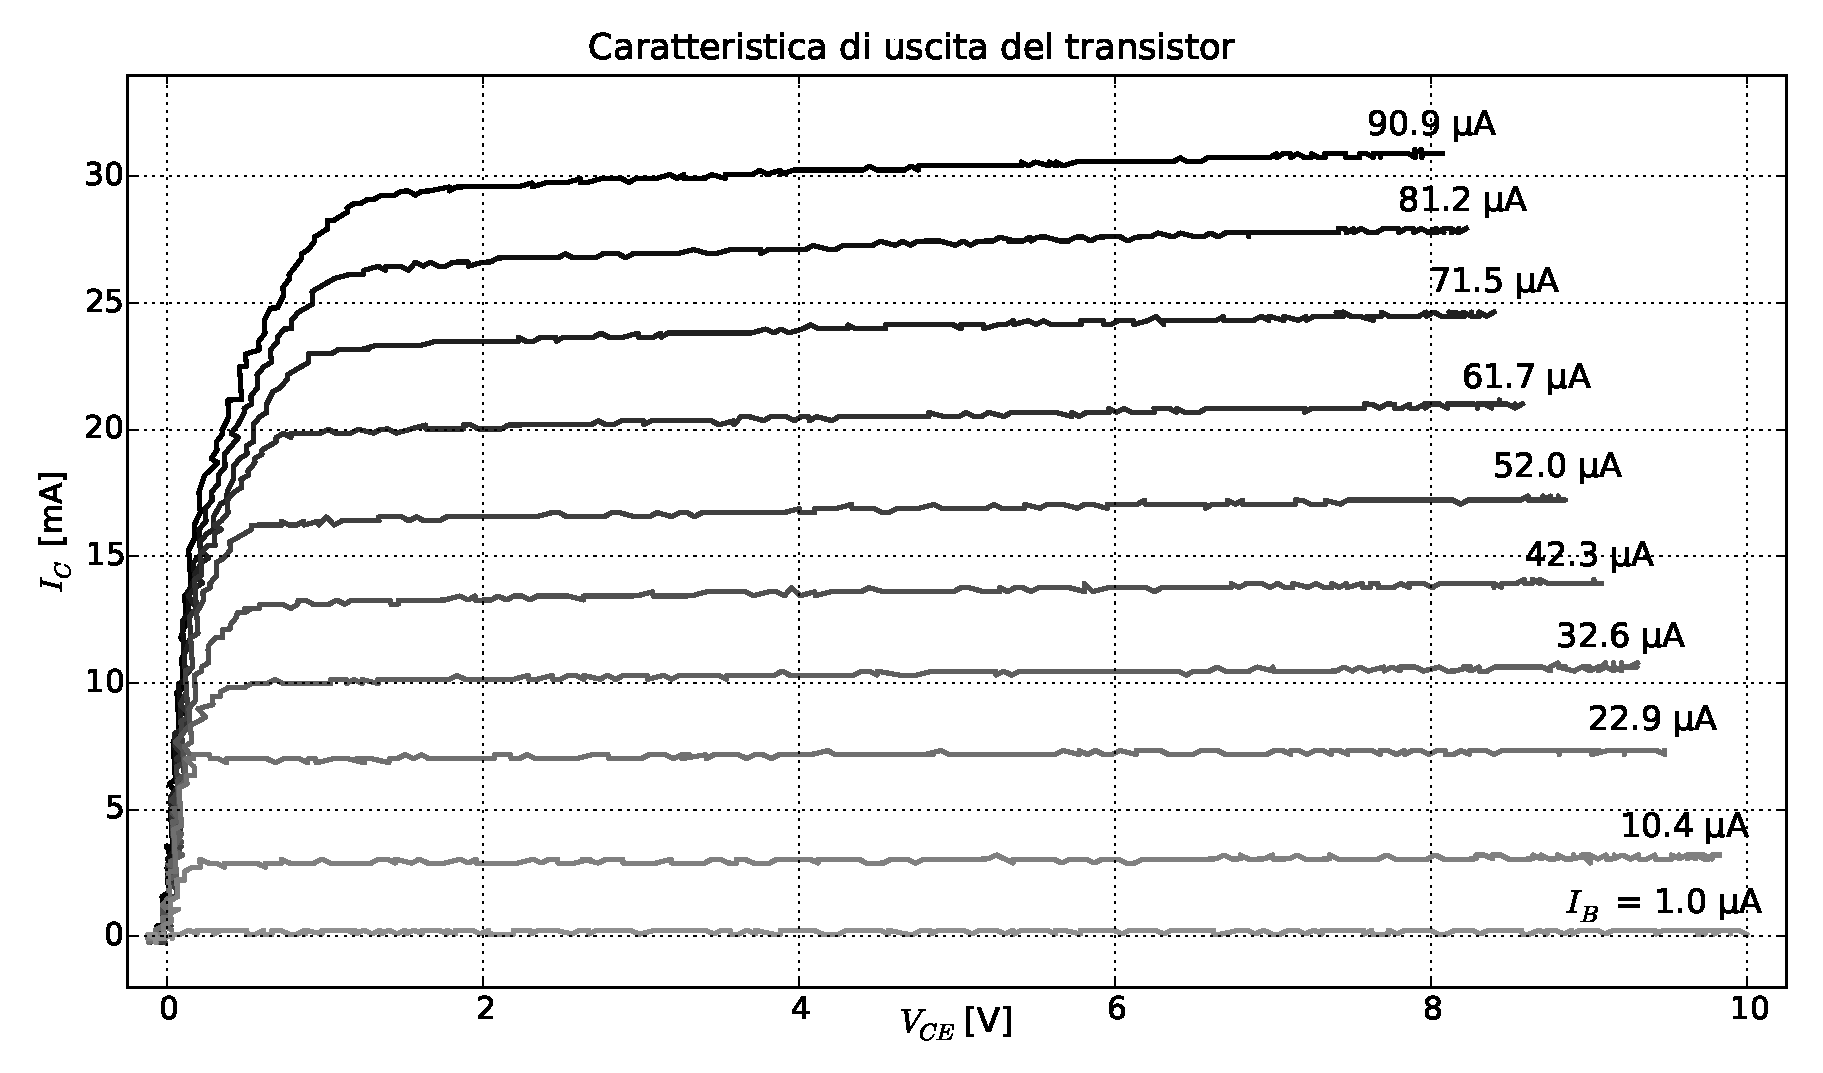
\includegraphics[scale=0.45]{xy.pdf}
	\label{fig:xy}
\end{figure}